\documentclass[12pt]{article}

\usepackage[margin=1in]{geometry}
\usepackage{amssymb}
\usepackage{amsmath}
\usepackage{graphicx}
\usepackage{subcaption}
\usepackage{cleveref}       % this package must be loaded at the last

\setlength{\parskip}{1em}


\newenvironment{question}[2][Question]{\begin{trivlist}
\kern10pt
\item[\hskip \labelsep {\bfseries #1}\hskip \labelsep {\bfseries #2.}]}{\end{trivlist}}


\begin{document}

\title{DD2424 Deep Learning in Data Science Assignment 4}
\author{Lin Chun Hung, chlin3@kth.se}

\maketitle

\section{Basic Part (Part 1)}

\begin{question}{i}
I used the central difference method to calculate the numerical gradients
with respect to all the network parameters and used it check against with the
analytical gradients.

I checked the maximum relative error which was mentioned in assignment and I 
used the numpy function \texttt{numpy.testing.assert\_allclose} to test if 
the gradients calculated analytically and numerically are closed element-wise.
During this time, the RNN model was set to be calculated in double precision. 

For the maximum relative error, only the \texttt{grad\_output\_wgt} went up to 
0.033. I think it is okay as the numerical gradient is calculate after the non-linear
activation layer. Other gradient maximum relative errors are pretty low and 
which are expected.

For the test assertion, consider the following equation:
\begin{equation*}
    % absolute(a - b) <= (atol + rtol * absolute(b))
    |a - b| \leq (\texttt{atol} + \texttt{rtol} * |b|)
\end{equation*}
where \texttt{atol} and \texttt{rtol} are the tolerance parameters.
In the assertion, I set \texttt{atol} to be 1e-3 and \texttt{rtol} to be 1e-4.

With these checking, I considered my analytical gradient calculations were bug free.
\end{question}

\begin{question}{ii}
I ran the training for 10 epochs, the smooth function is plotted in 
\cref{plt:smooth_lost_basic_rnn}.

\begin{figure}[h]
    \centering
    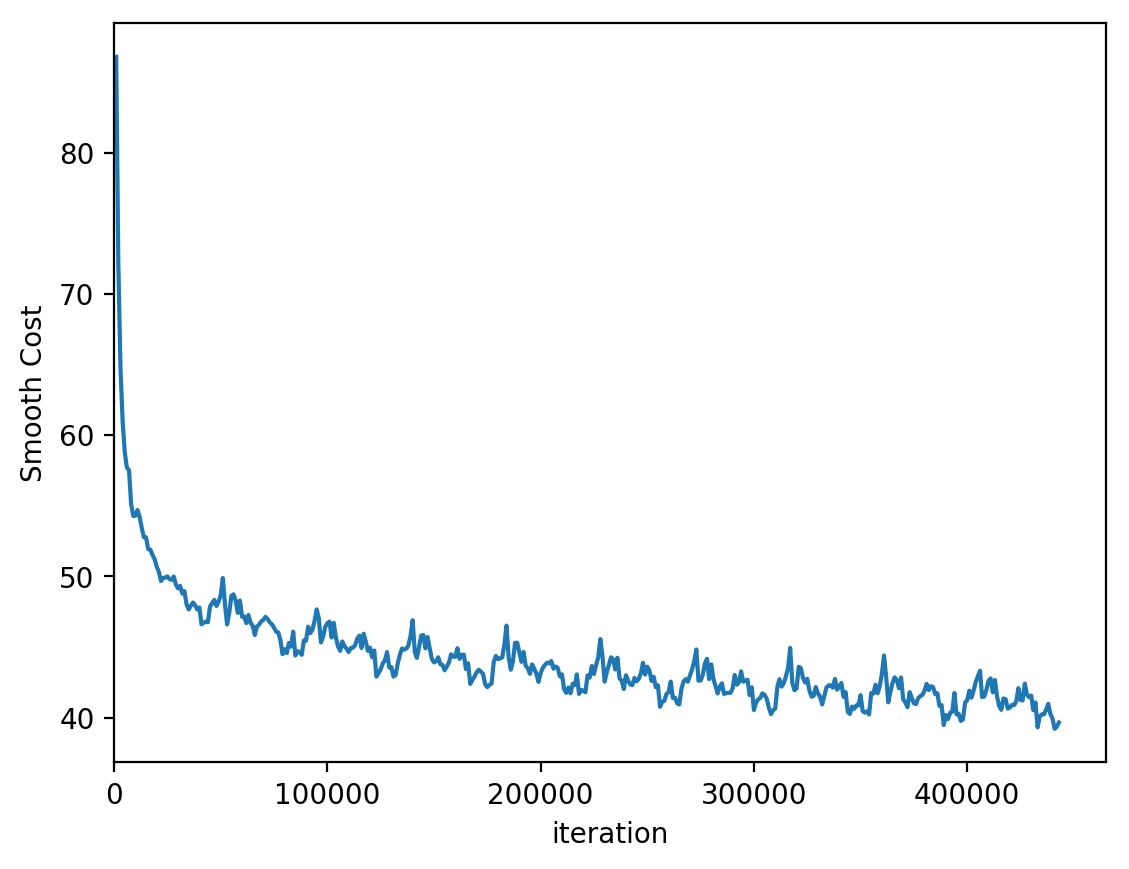
\includegraphics[width=0.8\textwidth]{./basic_cost.png}
    \caption{The smooth loss function plot}
    \label{plt:smooth_lost_basic_rnn}
\end{figure}
\end{question}


\end{document}
